\chapter{Regression}

\section{Problem}
Since there is no obvious regression problem for our data set, we need to manufacture one ourselves. The way we have chosen to accomplish this is to make an attempt at predicting one of the attributes based on the other attributes from a specified class. This means that we extract one of the attributes from our attribute set and make this our \texttt{y} vector.

\section{Forward selection}
% Apply linear regression with forward selection and consider if transforming
% or combining attributes potentially may turn useful. For linear regression
% plotting the residual error vs. the attributes can give some insight into whether
% including a transformation of a variable can improve the model, i.e. potentially
% describe parts of the residuals.
\begin{figure}[H]
\centering
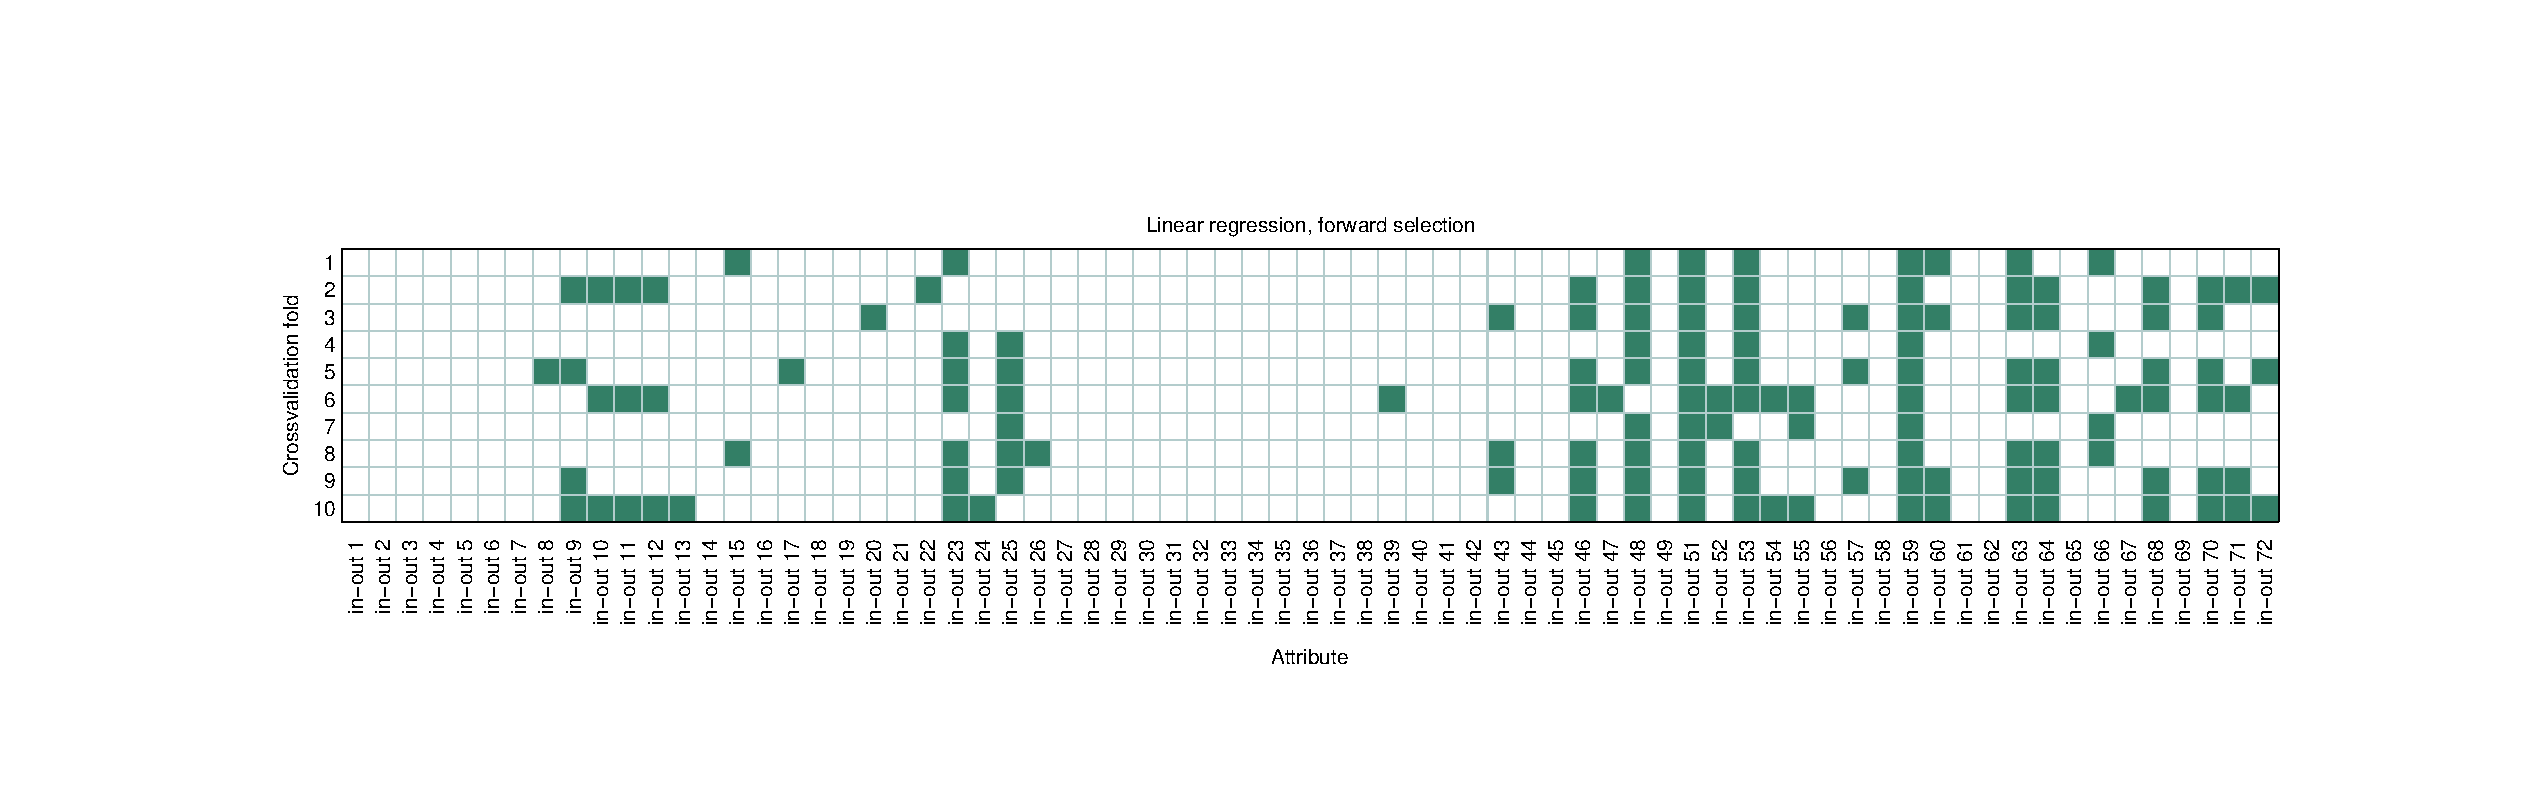
\includegraphics[width=\linewidth]{code/linear_regression_fs}
\caption{test\label{fig:linforward}}
\end{figure}

%\section{New data observation}
% Explain how a new data observation is predicted according to the estimated
% model. I.e. what are the effects of the selected attributes in terms of predicting
% the data.
% (Notice, if you interpret the magnitude of the estimated coefficients this in
% general requires that each attribute be normalized prior to the analysis.).


%\section{Artificial Neural Network}
% Fit an artificial neural network (ANN) model to the data.
% (You could consider only fitting the ANN to the attributes that were selected
% when you applied linear regression with forward selection).


%\section{Performance comparison}
% Statistically evaluate if there is a significant performance difference between
% the fitted ANN and linear regression models based on the same cross-validation
% splits (i.e., use a paired t-test). Compare in addition if the performance of your
% models are better than simply predicting the output to be the average of the
% training data output.